\taskpic{ Имеется равномерно заряженная диэлектрическая
  сфера. Известно, что, если ее разрезать пополам, то <<половинки>>
  будут расталкиваться с силой $F_1$. Если разрезать пополам одну из
  половинок (вдали от второй), то получившиеся <<четвертинки>> будут
  расталкиваться с силой $F_2$. И, наконец, если разрезать пополам
  одну из <<четвертинок>> (вдали от оставшихся частей сферы) на
  <<восьмушки>>, то они будут расталкиваться с силой $F_3$. Найти
  силу, с которой будут расталкиваться <<восьмушки>>, если их
  поместить так, как показано на рисунке.  }
{
  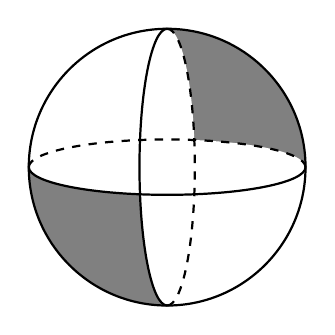
\begin{tikzpicture}
    \def\size{50pt}
    \draw [white,fill = gray]
		(0,0) -- (\size, 0) arc (0:90:\size) -- cycle;
    \draw [white,fill = gray]
		(0,0) -- (-\size, 0) arc (180:270:\size) -- cycle;
    \fill [fill = white] (0, \size) arc (90:270:\size / 5 and \size);
    \fill [fill = white, dashed]
    	(0, -\size) arc (-90:90:\size / 5 and \size);
    \draw [fill = white, dashed,thick]
    	(\size, 0) arc (0:180:50pt and \size / 5);
    \draw [fill = white,thick] (-\size, 0) arc (180:360:50pt and \size / 5);
	\draw [thick] (0, \size) arc (90:270:\size / 5 and \size);
    \draw [dashed,thick] (0, -\size) arc
    	(-90:90:\size / 5 and \size);
    \draw[thick] (0, 0) circle (\size);
  \end{tikzpicture}
}

